%%%%%%%%%%%%%%%%%%%%%%%%%%%%%%%%%%%%%%%%%%%%%%%%%%%%%%%%%%%%%%%%%%%%%%%%%%%
%% This file is part of the book
%%
%% Algorithmic Graph Theory
%% http://code.google.com/p/graph-theory-algorithms-book/
%%
%% Copyright (C) 2009--2011 Minh Van Nguyen <nguyenminh2@gmail.com>
%%
%% See the file COPYING for copying conditions.
%%%%%%%%%%%%%%%%%%%%%%%%%%%%%%%%%%%%%%%%%%%%%%%%%%%%%%%%%%%%%%%%%%%%%%%%%%%

\documentclass{article}

\usepackage{pgfplots}
\usetikzlibrary{external}
\tikzexternalize{graphs-as-plots}
\usepackage{subfigure}

\begin{document}

\begin{figure}
%% sin(x) and coordinates
\subfigure[Plots of functions.]{
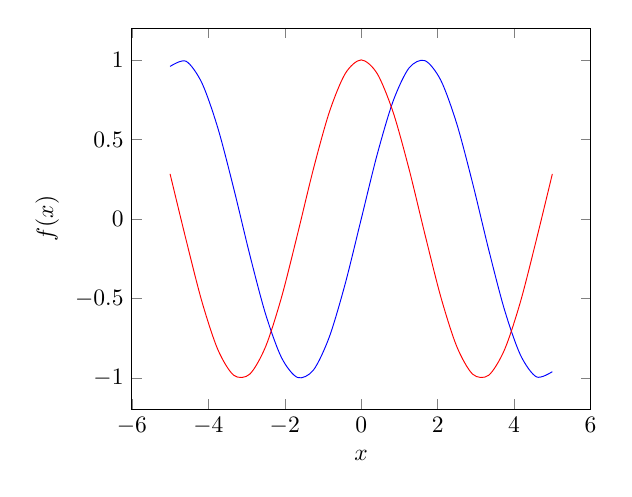
\begin{tikzpicture}
[scale=0.85]
\begin{axis}[%
  xlabel=$x$,%
  ylabel=$f(x)$%
]
%% The following works with Ubuntu 10.04, but does not work with
%% Ubuntu 10.10.
%% invoke external gnuplot as calculator
%% \addplot[smooth,color=blue] gnuplot{sin(x)};
%% \addplot[smooth,color=red] gnuplot{cos(x)};
%%
%% Equivalent of the previous block for Ubuntu 10.10.
\addplot[smooth,color=blue] expression {sin(deg(x))};
\addplot[smooth,color=red] expression {cos(deg(x))};
\end{axis}
\end{tikzpicture}
}
\quad
%%
%% scatterplot
\subfigure[A scatterplot.]{
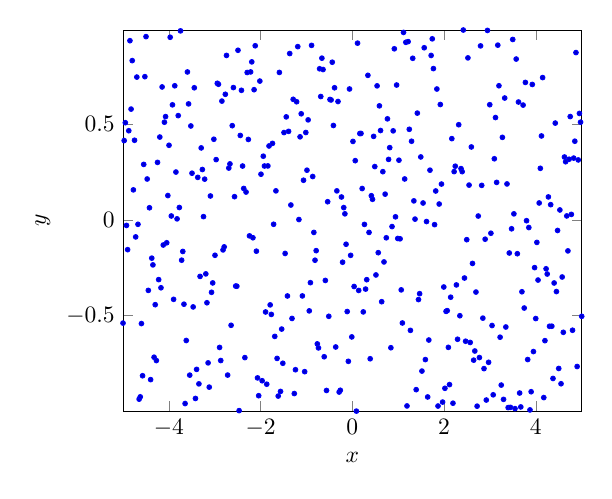
\begin{tikzpicture}
[every mark/.append style={scale=0.5},%
 scale=0.85]
\begin{axis}[%
  enlargelimits=false,%
  xlabel=$x$,%
  ylabel=$y$%
]
\addplot+[only marks,samples=400] {rand};
\end{axis}
\end{tikzpicture}
}
\end{figure}

\end{document}
